\subsection{$T_{20}$ Experimental Method} %Measurement of $A_{zz}$ }
\label{t20_exp}

A measurement of $T_{20}$ will be extracted from $A_{zz}$ on the elastic peak for each $Q^2$ mentioned in Section~\ref{kinematics}. We will follow the method described by the NIKHEF measurements~\cite{Bouwhuis:1998re}, which also used a tensor polarized target. Our methods differ in that we will use the high resolution of the HMS and SHMS to determine the elastic peak through kinematic cuts, where NIKHEF utilized a second spectrometer for that purpose. 
%It should also be noted that the Boden measurement used a beam current of $<0.4$~nA. The current for these proposed $T_{20}$ measurements at \CURRENT~nA is $200\times$ the exploratory Boden measurement.

The analyzing powers of a tensor-polarized target are described by the cross-section
\begin{equation}
\sigma = \sigma_0\left[ 1 + \frac{A_d^T P_{zz}}{\sqrt{2}} \right],
\label{cs-ana}
\end{equation}
where
\begin{equation} A^T_d = \sum_{i=0}^{2}d_{2i}T_{2i}
\end{equation}
and
\begin{equation} d_{20} = \frac{3 \cos^2 \theta^* -1}{2},~~d_{21} = -\sqrt{\frac{3}{2}}\sin2\theta^*\cos\phi^*,~~d_{22}=\sqrt{\frac{3}{2}}\sin^2\theta^*\cos 2\phi^*.
\end{equation}
$\theta^*$ and $\phi^*$ are in the frame where the $z$ axis is along the $\vec{q}$ and the $x$ axis is perpendicular to $z$ in the scattering plane, as described in~\cite{Donnelly:1985ry} and shown in Fig.~\ref{coords}. For this proposal, $\theta^* \approx 70^{\circ}$ and $\phi^* \approx 0^{\circ}$, as our target field will be oriented along the beamline and $\theta_{\vec{q}}\approx 70^{\circ}$ on the elastic peak.

\begin{figure}
\begin{center}
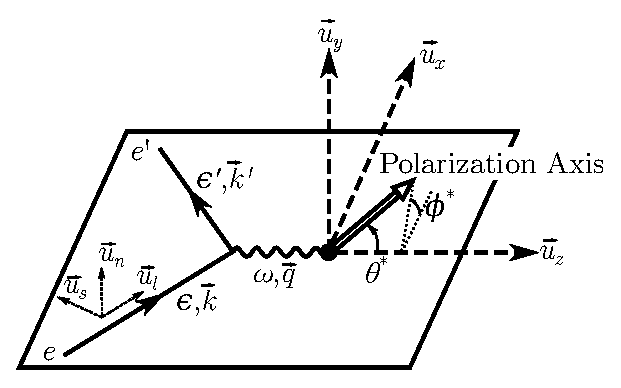
\includegraphics[width=0.4\textwidth]{figs/coordinate_system.eps} 
\caption{\label{coords}Coordinate system used in determining the tensor analyzing powers.
}
\end{center}
\end{figure}

%If that's the case, the $d_{21}\approx -0.787,~~d_{22}\approx 1.08~~$ and $d_{20} \approx -0.3245$.

We rearrange Eq.~\ref{cs-ana} to be defined as our observable $A_{zz} = \frac{2}{P_{zz}}\left( \frac{\sigma}{\sigma_0} - 1 \right)$,
\begin{equation}A_{zz} = \sqrt{2} \left[ d_{20} T_{20} + d_{21} T_{21} + d_{22} T_{22}\right],
\end{equation}
\begin{equation}
T_{20} = \frac{A_{zz}}{d_{20}\sqrt{2}}-\frac{d_{21}}{d_{20}}T_{21}-\frac{d_{22}}{d_{20}}T_{22}.
\end{equation}
Contributions from $T_{21}$ and $T_{22}$ are expected to be small but not negligible, and will be calculated from models that best match world data. Uncertainties from $T_{21}$ and $T_{22}$ are expected to be $10\%$ and are included within the $T_{20}$ systematic calculations.


